%\documentclass[4pt,a4paper]{article}
\documentclass[4pt,a4paper,twocolumn]{article}
\usepackage[utf8]{inputenc}
\usepackage[english]{babel}
\usepackage{algorithm}
\usepackage{textcomp}
\usepackage{fontenc}
\usepackage{tipa}
\usepackage{framed}
\usepackage{multicol}
\usepackage{color}
\usepackage{graphicx}
\usepackage{amsmath}

\usepackage{cite}
\usepackage{lastpage}
\usepackage{lmodern}




\usepackage[]{hyperref}
\hypersetup{  
	colorlinks=true,
    urlcolor=cyan           % color of external links
}

\author{David Przybilla\\dav.alejandro@gmail.com, davida@coli.uni-saarland.de\\ \\ Term Paper for Knowledge Representation Seminar\\ Universit\"{a}t des Saarlandes}
\title{Automatic Generation of Knowledge Representation}
\begin{document}
\twocolumn[
	 \begin{@twocolumnfalse}
    \maketitle
  \end{@twocolumnfalse}
 ]




\section{Introduction}


\begin{figure*}[]
  \centering
    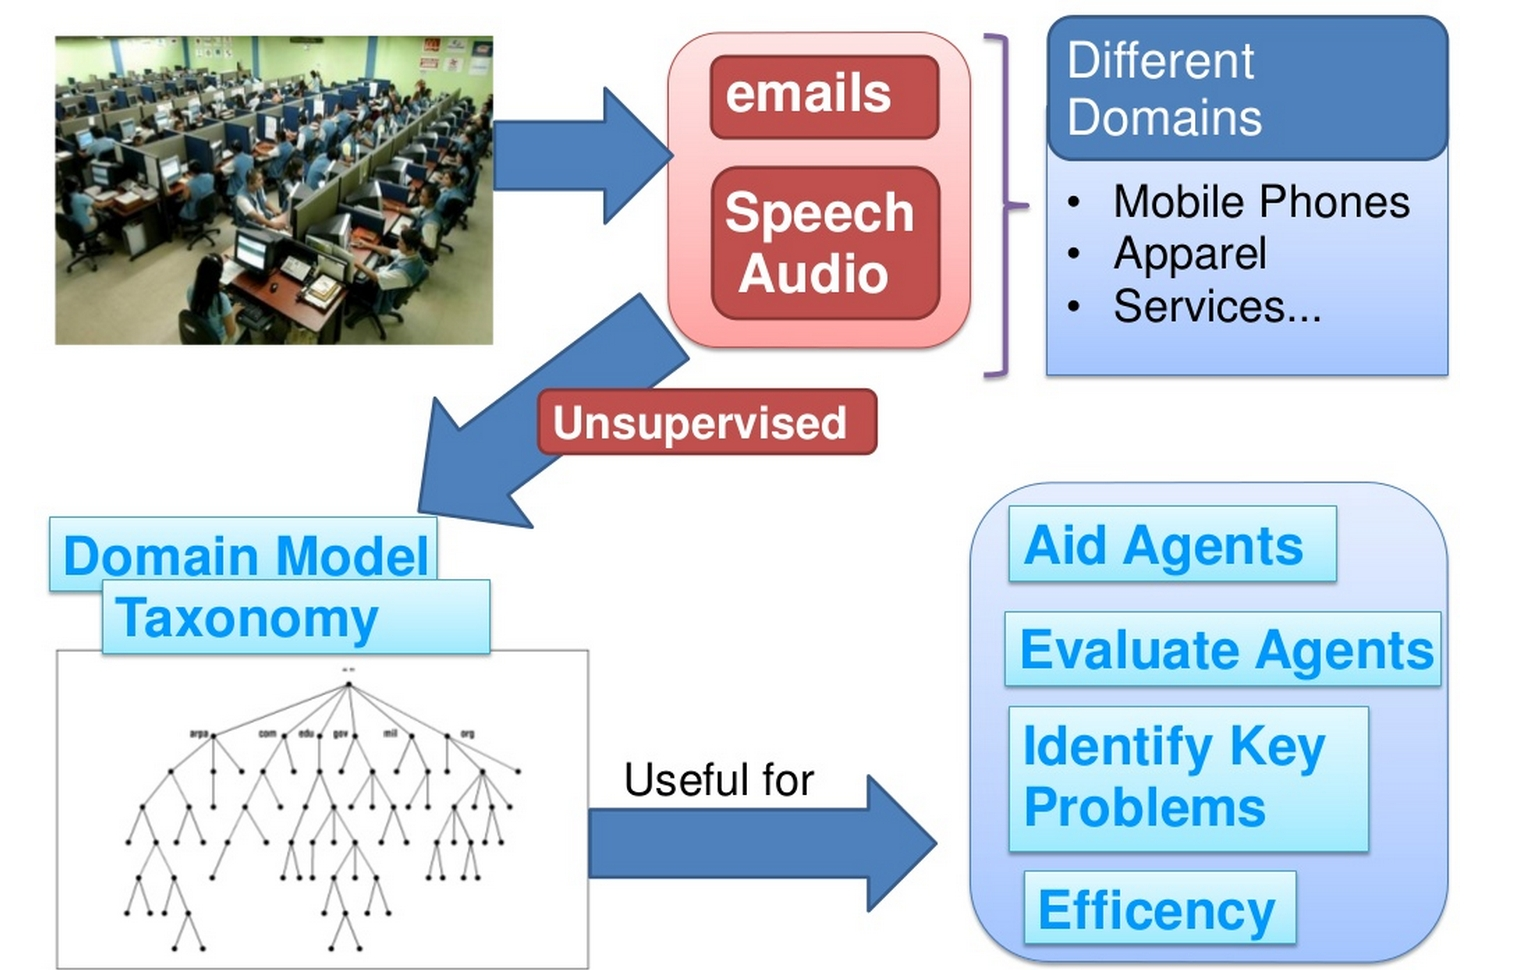
\includegraphics[scale=0.2]{pics/problem.jpg}
    \caption{Problem Diagram}
   \label{fig:problem}  
\end{figure*}

This report focus on the paper \textit{Automatic Generation of Domains Models for call centers from noisy transcriptions} ~\cite{Roy:2006:AGD:1220175.1220268}.\\
In the given paper the authors describe a method for automatically creating a taxonomy.\\
The domain of the problem are the issues of a Callcenter. The Call center handles user problems related to different sofware and services.\\
The proposed method use  written and speech records between the agents of the call center and the clients to built the ontology. \\
In the next sections  the method for transforming unstructured data into a knowledge representation proposed by the paper will be described,
then a critical review and opinion over the method will be given. Additionally a comparison between the given paper and other papers willing to automatically construct knowledge representation is made.
The last section covers  possible applications of automatically constructed Ontologies in the domain of Natural Language Processing.

\section{Motivation}

Automatically creating knowledge representation from unstructured text has been a focus of study given the amount of data available in the web.
Projects such as 'Know it all'\footnote{\url{http://www.cs.washington.edu/research/knowitall/}} considers the problem of developing a variety of domain-independent systems that extract information from the Web in an autonomous, scalable way.\\ Google\footnote{\url{http://www.google.com/insidesearch/features/search/knowledge.html}} for example has the project 'The knowledge Graph' which considers the automatically construction of an ontology by using the web knowledge. \\
\\
Nevertheless the unstructured nature of the information has proven to be an challenge when constructing knowledge representations, natural languages arises many problems when trying to understand their semantics and to abstract concrete cases into general relations and entities.\\
In the opinion of this reviewer Information Extraction provided a first simple task into automatically creating structures from natural language texts. The task in information extraction consist in gathering  relations among entities from raw text.\\
In the first stages of this task only a very specific range of relations and entities are to be caught.
For example one would like to gather all relations and entities talking about  "getting the nobel prize" or "change of chairs in a company".\\
However in the recent years this trend has evolved towards "Open Information Extraction", which wants to capture as much as entities and relations as possible given raw text.\\
The applications to information extraction are countless, the ouput of the task provide a resource for other more sophisticated processes, and it could be useful for example to topic mining, opinion mining or information retrieval or to correlate different relations or events captured from different sources.
In the opinion of the reviewer this provides a first step into building an ontology, since it would allow initially to have a candidate pool of concepts and relations.\\
\\
During the last years focus has been put into strategies which allow to capture structures in raw text, for example Cortez and Oliveira ~\cite{Cortez:2011:JUS:1989323.1989380} proposed a method for extracting data from semistructured texts. In their experiments their system learns without human intervention the structures in which Cooking recipes are written and it is able to match each step and ingredients of the recipes into a structured representation.\\
This could be a major improvement since it would allow for example to capture entities and relations from soruces of knowledge that are semi-structured like Wikipedia.\\
\\
Addionally The reviewer would like to mention that even though there is a focus on creating Ontologies, there is also a focus on Extending the current ones in an automatic way.\\
Many tasks require Knowledge sources in order to achieve good performance, however this depends deeply on the coverage of the Knowledge representation. 
Consider for example the applications using Wordnet or Framenet, they heavily rely on the coverage of those sources to disambiguate the senses of the words.
In ~\cite{Tonelli:2013:WWM:2405838.2405917} Tonelli proposes a method for extending this Knowledge Sources by using Wikipedia in a semi-automatic way.
Following the same trend Yamada ~\cite{yamada-EtAl:2011:IJCNLP-2011} tries to extend Wordnet in an automatic way by using Wikipedia.\\
Following a different direction Pinkal,Regneri and Koller  in ~\cite{regneri-koller-pinkal:2010:ACL} propose the use of crowdsourcing to gather scripts of common activities (like shopping, cooking and egg) in order to model $Common\, Knowledge$ which is often overlooked by computer systems.


\section{Preprocessing }
As an initial step to start the process of creating the taxonomy a preprocessing step is proposed by the paper.\\
In the preprocessing two major steps take place, first the Speech Data is transformed into text and second the text is transformed into feature vectors for the method incharged of building the taxonomy.



\subsection{Automatic Speech Recognition}
		
During this step the conversations between agents and clients which have been recorded are transformed into text using Automatic Speech Recognition.\\
The authors of the paper mention that they transformed more than 2000 calls  but they never mention the ratio of already given transcriptions to the generated transcriptions using Speech Recognition.\\
The authors also describe several issues that they identified for this step, they actually claim that the data generated during this process is very noisy with an error rate of about 40\%.\\
Some of the issues are:
\begin{itemize}

	\item Different Accents: Since the call center takes calls from all over the world, the speakers usually have different access. The tool they used for ASR seems to be affected by this fact.
	
	\item Deletion of Words 
	
	\item Wrong words are inserted
	
	\item Wrong Speaker is assigned
	
	\item no punctuation marks
	
	\item silence periods
	
	\item no sentence boundaries
	
	\item false starts
	
	\item filling words (i.e : "um", "uhh")
\end{itemize}

For the reviewer of this paper is unclear whether this are actually issues.\\
First there is no clear view of the proportion betweet transcript data and the data generated by the speech recognition step, that is, if the proportion is very small it would not matter at all.\\
Secondly given the BoW(Bag of Words) approach they use in their system later, is irrelevant that the wrong speaker is assigned, or whether there is punctuation marks or not. Moreover I would speculate that having wrong words inserted or deletions of words should not be so painful for the performance of their system. I will explain this phenomena by the end of the next subsection.


\subsection{Feature Engenieering component}

This corresponds to the second step of the preprocessing. In this step the texts are pruned and transformed into feature vectors (Figure ~\ref{fig:eng_component} ).\\
Each document pass through the following filters:

\begin{figure*}[]
  \centering
    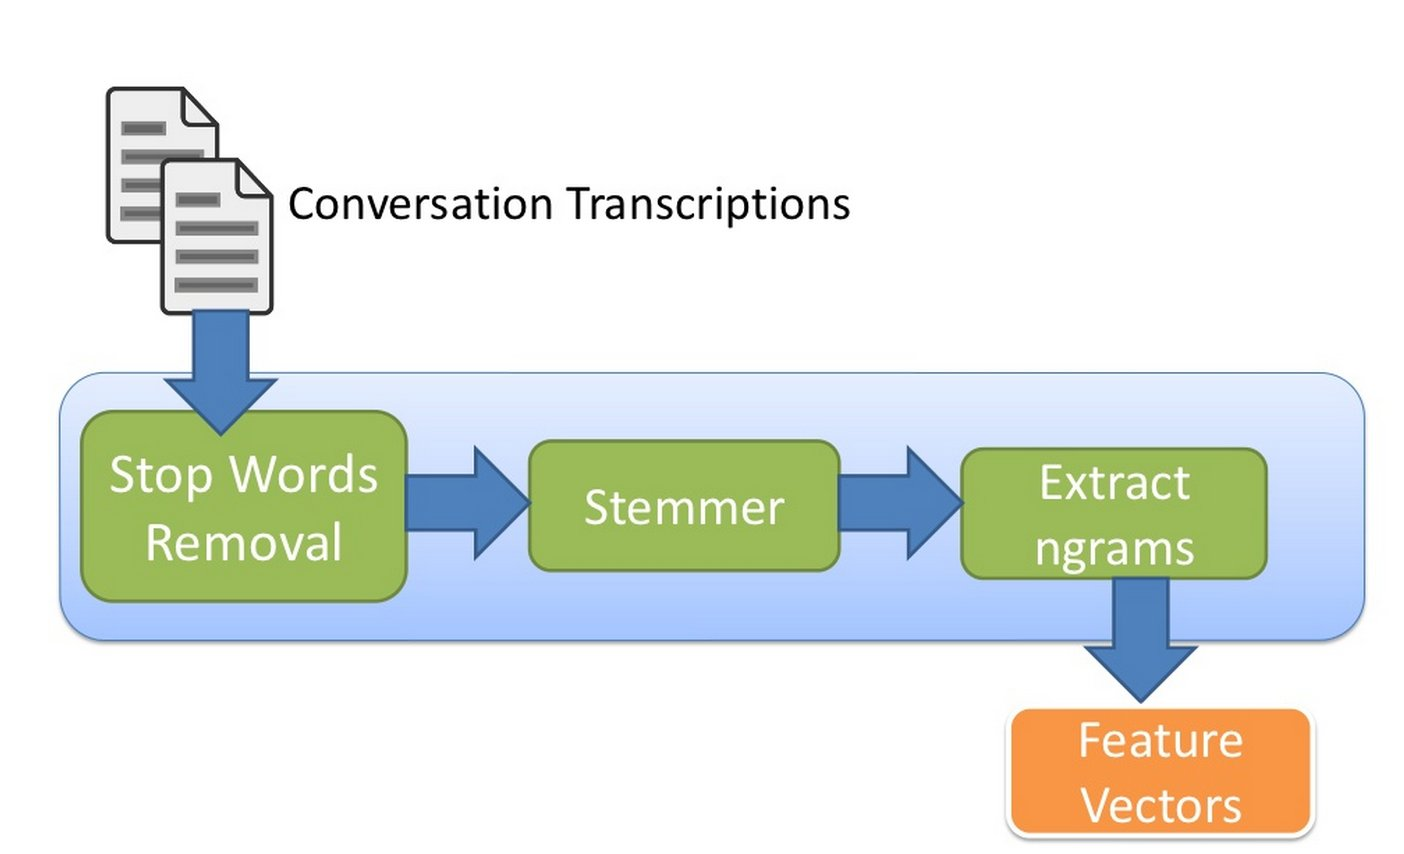
\includegraphics[scale=0.2]{pics/eng_component.jpg}
    \caption{Feature Engenieering component}
   \label{fig:eng_component}  
\end{figure*}

\begin{itemize}
	\item Stop Word Removal: Functional words which do not convey relevant meaning are removed (i.e: ''for",''of"..).
	
	\item stemmer: Each word is converted into its stem. This has the objective of aligning dimensions in the following process for building the taxonomy.
	
	\item extract ngrams:  generate a feature vector of each document with Ngrams.
\end{itemize}

For the reviewer all of the filters mentioned should be ok given that the taxonomy builders require text clustering.\\
Nevertheless the previous mentioned noisy inclution by the ASR system could be objected as follows:

\begin{itemize}
	\item Conversations are long enough. Conversations of this kinds are long enough for keywords to be repeated several times during the conversations, that is, even if there is word deletion the system would have several opportunities to capture the right keywords, the other words which are not likely to be keywords will be discarded by the system anyway.

  \item Given the BoW approach, the wrong word insertion would only harm when they inserted word is a domain keyword.
  
\end{itemize}

For the reviewer further steps could be done given that the creation of the taxonomy relies on Text clustering.\\
It should be possible for example to extend each document with extra keywords in order to have a better dimension aligment.This have been done in solving tasks such as  textual entailment ~\cite{Mirkin:2009:EIU:1609067.1609129} where hypothesis have been extended using Wordnet,framenet and other sources of knowledge. This strategy has also been used in text clustering of short texts (i.e: tweets)  in order to gain coverage and recall, in ~\cite{Gabrilovich:2006:OBB:1597348.1597395} Gabrilovich proposes a strategy for extending tweets with words from Wikipedia.\\
The call center could for example use keywords from the manual of the software they support.


	\section{Creating the Taxonomy}
		\subsection{Clusterer}
		\subsection{Taxonomy Builder}
		\subsection{Model Builder}


	\section{Asessing the results}

	

Discussion

Issues regarding the assesment

Issues with NLP processing used

what is this representation useful for? QA?

Comparison with other papers using nlp to generate knowledge representation







\bibliography{paper}{}
\bibliographystyle{alpha}






\end{document}


